\section{Filtering the test signal for directionality measurement}\label{sec:signal_filtering}
For the sake of simplicity, when measuring the polar response of the speaker array as described in \autoref{ax:directional_3}, the filtering is done offline and the measurement routine is fed different signals as reference and outputs. These are achieved by generating a sweep in MATLAB and then using the \texttt{filter} function to apply the filters, that have been developed in \autoref{sec:filter_design}. The resulting signals are stored as wave files and are therefore normed so that there is no value bigger then 1.
The upper envelope of the sweep time signals is illustrated in \autoref{fig:time_signals}.
\begin{figure}[H]
	\centering
	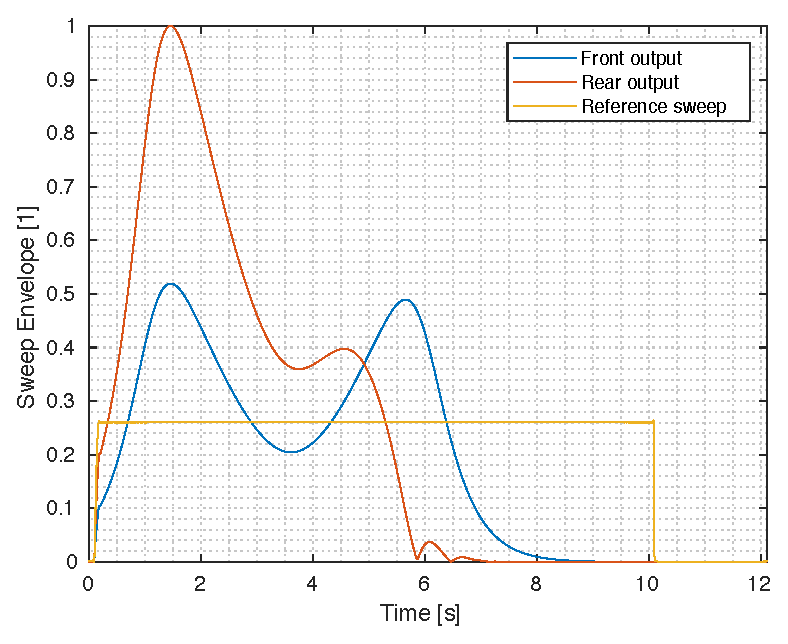
\includegraphics[width=0.7\textwidth]{time_signals.eps}
	\caption{Upper envelope of sweeps for array polar response measurement}
	\label{fig:time_signals}
\end{figure}


\section{Conclusion on Measurement Preparation}
With the formerly disclosed construction, it is possible to set up a loudspeaker array according to the requirements for the placement of the acoustic centers from \autoref{ssec:cost_map}. The setup is mostly suited to a laboratory environment as it requires careful adjustments before any measurement or demonstration. Account for adjustments in the construction should enable the contraption to be suitable for a variety of array dimensions. For the measurement routine, the swept sine signal is done offline and therefore the filtering part is also only suited for laboratory environment.
%It can be concluded that it was possible to make a stable speaker measuring stand where all three speaker can be allined and adjusted and still be a stable construction.